\documentclass[conference]{IEEEtran}

%%%%%%%%%%%%%%%%%%%%%%%%%%%%%%%%%%%%%%%%%%%%%%%%%%%%%%%%%%%%%%%%%%%%%%%%%%%%%%%%
%
% Package
%
%%%%%%%%%%%%%%%%%%%%%%%%%%%%%%%%%%%%%%%%%%%%%%%%%%%%%%%%%%%%%%%%%%%%%%%%%%%%%%%%
\usepackage{ifpdf}
\ifCLASSINFOpdf
  \usepackage[pdftex]{graphicx}
  % declare the path(s) where your graphic files are
  % \graphicspath{{../pdf/}{../jpeg/}}
  % and their extensions so you won't have to specify these with
  % every instance of \includegraphics
  \DeclareGraphicsExtensions{.pdf,.jpeg,.png}
\else
  % or other class option (dvipsone, dvipdf, if not using dvips). graphicx
  % will default to the driver specified in the system graphics.cfg if no
  % driver is specified.
  \usepackage[dvips]{graphicx}
  % declare the path(s) where your graphic files are
  % \graphicspath{{../eps/}}
  % and their extensions so you won't have to specify these with
  % every instance of \includegraphics
  \DeclareGraphicsExtensions{.eps}
\fi

\usepackage[utf8]{inputenc}
\usepackage[T1]{fontenc}
\usepackage[french, english]{babel}
\usepackage{cite}
\usepackage{caption}
\usepackage{amsmath,amsfonts,amssymb}
\usepackage{subcaption}
\usepackage{array}
\usepackage{float}
\usepackage{multicol}
\usepackage{algpseudocode}
\usepackage{algorithm}


\begin{document}
\pagestyle{plain}
\title{Control of Prosumer Networks}


\author{Nicolas Gensollen, Monique Becker, Vincent Gauthier and Michel Marot  \\
\IEEEauthorblockA{CNRS UMR 5157 SAMOVAR, \\
Telecom SudParis/Institut Mines Telecom\\
Email: \{nicolas.gensollen, vincent.gauthier, michel.marot, monique.becker\}@telecom-sudparis.eu}}


\maketitle


\begin{abstract}
The ability to control a given network by  dynamically injecting inputs offers ways to make sure that it stays in stable regions. In the case of smart grids, where end users exhibit complex behaviors and renewable production is quite unstable, control of the system  is paramount. In this paper, we study the case of a network composed of entities called prosumers. These agents have the ability to both consume and produce according to external conditions. We first model and simplify the underlying dynamic of such network using a second order coupled oscillators network model. Under some conditions, the system synchronize to a common frequency. However, in case of perturbations in the power distribution, the system might lose synchrony and require control to bring it back to the stable state. In this situation, control can be seen as energy  absorbed or injected in the system at specific locations. Moreover, the power outputs of the prosumers are susceptible to change such that loads and generators are not fixed. In this context, it is important to select the right subset of nodes that yields, on average, the cheapest control in terms of energy. 
\end{abstract}


\IEEEpeerreviewmaketitle


\section{Introduction}
\label{sec:introduction}

Modernizing the power grids and increasing the share of renewables in the production are two substantial objectives of the energetic transition. Because of parallel progresses in communication, data management, and storage, the upcoming emergence of a power grid "2.0", often called smart grid, appears as a cross-disciplinary challenge of the 21st century \cite{Ramchurn}.

It is believed that these new ways of producing and managing energy, will also impact how end users consume. More precisely, the consumer   of the future is expected to be more involved in the system operation. Using dynamic signals (real time electricity prices for instance), load curves could be shaped to some extend as to agree with the production conditions of the main grid.
Furthermore, the emergence of renewable distributed energy resources (DER) in the distribution networks, possibly hold by individuals,
will completely modify the today end user agent model.

These new agents that can both consume and produce are often called prosumers \cite{Rathnayaka2012}. This decentralized production is believed to lead to more resilient systems than today centralized power grid. Nonetheless, the difficulty of dealing with decentralized production is coupled with the high uncertainty of renewables. Ensure system stability in these conditions appears thus as a complex task. 

Relying on the ability of the smart grid to obtain, communicate and analyse data, several solutions could  improve the stability of such complex systems. Among these solutions, demand side management and energy storage are two of the most popular ones. In this paper, we explore the use of storage in a network of prosumers whose power outputs are susceptible to change due to various external causes. More precisely, we are interested in the "best" locations for the storage equipments such that we are able to maintain stability when  perturbations occur. Since all nodes can switch from generator to load and vice versa, the optimal location is susceptible to change with the prosumers power output.
Our goal is then to find the one that, on average, provide the best results.

Since charging and discharging a battery is costly, we are particularly interested in the energy necessary to control the system when perturbations occur. The notion of performance of a given set of locations for using storage would then be inversely proportional to the energy used. One problem with this definition is that it depends explicitly on the state of the system and the prosumers power distribution. Besides, as the system size increases, the number of possible location sets increases exponentially. This forbid any algorithms using complete enumeration and evaluation of the sets. Moreover, we consider  that the electrical lines have maximum capacities, and storage equipments have both a maximum charge / discharge rate and  bounded capacities. Obviously, only solutions satisfying these constraints will be considered as feasible.

 In this paper, we model the prosumer network as a coupled oscillator network. Inspired by \cite{Filatrella2008}, we use a second order Kuramoto model that can be seen as a simplified version of the underlying power grid dynamics (see Section \ref{sec:The_Model}). We then use control theory \cite{Liu2015} in order to model the impact of the storage equipments on the network (see Section \ref{sec:control_and_submodularity}). Using the relationships between submodular set functions and the Gramian matrix \cite{Summers2014}, we use a modified version of a greedy algorithm \cite{Minoux} in order to find the smallest locations set that minimizes the average control energy while satisfying all the constraints (see section \ref{sec:Control_prosumer}). Finally, we show some results in Section \ref{sec:Results}.


\section{The Model}
\label{sec:The_Model}

In this section, we introduce the coupled oscillators network model used to simplify the power grid dynamic. The detailed derivation of the second order dynamics can be found in \cite{Filatrella2008}, and the key points are reproduced here for the convenience of the reader.

 The objective is to achieve synchronization of the grid at the main frequency $ \Omega = 50 Hz $. Each oscillator i has a phase angle $ \delta_i $ and a frequency $ \dot{\delta}_i $. Therefore, we seek an equilibrium of the form : $ \forall i,\ \dot{\delta}_i = \Omega $. For convenience, we express the dynamic of the oscillators in terms of the deviations from the main frequency : $ \delta_i(t) = \Omega t + \theta_i(t) $. Let $ \omega_i = \dot{\theta_i} $, such that $ \dot{\delta_i} = \Omega + \omega_i $. The equilibrium, in terms of the deviations dynamics, is : $ \forall i,\ \omega_i = 0 $

The next step consists in translating the dynamics of the generators and machines into equations involving the phase angles $ \theta_i $ and the frequencies $ \omega_i$. Generators and machines are composed of a turbine that dissipates energy at a rate proportional to the square of the angular velocity ($P_{diss} = FV \sim V^2 $ ) : 

\begin{equation}
  P_{diss, i}(t) = K_{Di}(\dot{\delta_i}(t))^2 
\end{equation}

where $ K_{Di} $ is the dissipation constant of entity i.

Furthermore, it also accumulates kinetic energy at a rate : 

\begin{equation} 
P_{acc,i}(t) = \frac{1}{2}I_i\frac{d}{dt} \left( \dot{ \delta_i }(t)^2 \right)
\end{equation} 

where $ I_{i}$ is the moment of inertia of entity i. For simplicity, we consider that all entities have the same dissipation constants($K_D$) and moment of inertia (I).

The condition for the power transmission between i and j is that the two devices do not operate in phase : The phase difference between i and j is : $ \delta_j(t) - \delta_i(t) = \Omega t + \theta_j(t) - \Omega t - \theta_i(t) = \theta_j(t) - \theta_i(t) $.

The transmitted power along the line can thus be written as : 

\begin{equation}
 P_{transmitted} = - P_{ij}^{MAX} sin( \theta_j - \theta_i )
\end{equation}
  
with $ P_{ij}^{MAX} $ being the maximum capacity of the line $(i,j)$. If i is connected to more than one other entities, this equation becomes ($\mathcal{N}_i$ being the neighborhood of  i) : 

\begin{equation}
  P_{transmitted} = - \sum_{j \in \mathcal{N}_i} P_{ij}^{MAX} sin( \theta_j - \theta_i ) 
\end{equation}


Each entity i is then described by a power balance equation of the type :

\begin{equation}
 P_{S,i}  =  P_{diss,i} + P_{acc,i} + P_{transmitted,i} 
\end{equation}

By substituting and re-arranging the terms, we obtain the following non-linear coupled system of equations :

\begin{equation}
\begin{array}{lll}
P_{S, i}  =  I \Omega \ddot{ \theta_i }  + \left[ I \ddot{ \theta_i } + 2 K_D \Omega \right] \dot{ \theta_i } + K_D \Omega^2 \\+ K_D \dot{ \theta_i }^2 - \sum_{j \in \mathcal{N}_i} P_{ij}^{MAX} sin \left[ \theta_j - \theta_i \right] \end{array}
\end{equation}

These non linear equations are obviously not very practical. We now use some approximations based on the fact that we consider only small deviations from the main frequency : $ \dot{ \delta}_i \sim \Omega $ which means that $ \omega_i = \dot{\theta_i} << \Omega $, such that the squared term $ K_D \dot{\theta}_i^2 $ can be neglected.
Moreover, we assume that the rate at which energy is stored in the kinetic term is much less of the rate at which energy is dissipated by friction, a common condition for mechanical systems : $ \ddot{ \theta }_i  << \frac{2 K_D}{I} $

The equation can thus be simplified to :

\begin{equation}
 \ddot{ \theta_i } \sim \psi_i - \alpha \dot{ \theta_i } + \sum_{j\neq i} K_{ij} g_{ji} sin \left[ \theta_j - \theta_i \right] 
\end{equation}

Where $ \alpha = \frac{2 K_D}{I} $ is the dissipation term, $ K_{ij} = \frac{P_{ij}^{MAX}}{I \Omega} $ are the coupling strengths, $ \psi_i = \left[ \frac{P_{S,i}}{I \Omega} - \frac{K_D \Omega}{I} \right] $, and $ g_{ij} $ is the coefficient of the adjacency matrix G.
By working in a rotating frame, we can simplify $ \psi_i=\frac{P_{S,i}}{I \Omega} $.

The dynamic is still non linear because of the sine coupling. Therefore, we also assume that the phase angle differences are small such that $ sin \left[ \theta_j - \theta_i \right] \sim \theta_j - \theta_i $. By using vector notations, the dynamic can be written in the following form :

\begin{equation}
\ddot{\theta} = \Psi - \alpha \dot{\theta} - KL\theta
\end{equation}

Where L is the Laplacian matrix of the underlying topology ($ k_i $ is the degree of node i):

\begin{equation}
L_{ij} = \left\{ \begin{array}{lll} k_i\ \ \ \ \,if\ i=j \\ -g_{ij}\  if\ i \neq j \end{array} \right. 
\end{equation}


This is a continuous time second order linear system of $ N $ equations. We first transform this into a continuous time first order linear system of $ 2 N $ equations by introducing the following vector : $ X = \left( \begin{array}{c} \theta \\ \dot{\theta} \end{array} \right)$ : 

\begin{equation}
 \dot{X} = \left( \begin{array}{cc} 0 & I \\ - KL & -\alpha I \end{array} \right) X + \left( \begin{array}{c} 0 \\ \Psi \end{array} \right)
\end{equation}
 
Which can be written in discrete time: 

\begin{equation} 
X(t+\Delta t) = M  X(t) +  \left( \begin{array}{c} 0 \\ \Psi \Delta t \end{array} \right)
\end{equation} 

With $ M = \left( \begin{array}{cc} I & I \Delta t \\ -KL \Delta t & (1-\alpha \Delta t) I \end{array} \right) $.

By setting $ Y(t) =  \left( \begin{array}{c} X(t) \\ 1 \end{array} \right) $, let the dynamic be :

\begin{equation}
 Y(t+\Delta t) = A Y(t)
\end{equation}

With transition matrix A :

\begin{equation}
 A =   \left( \begin{array}{ccc} I & I \Delta t & 0 \\ -KL \Delta t & (1-\alpha \Delta t)I & \Psi \Delta t \\ 0&0&1 \end{array} \right)
\end{equation}

This is a linear discrete time system of $ 2 N + 1 $ equations. Note that the transition matrix A encodes all the system parameters, topology, and power distribution.



\section{Control and Submodularity}
\label{sec:control_and_submodularity}

\subsection{Submodularity}

In this section we provide a very brief introduction to what submodular functions are, and how their maximization could be achieved in reasonable time. More information can be found in \cite{Krause2014}.

 A set function $ F:2^{V} \longrightarrow \Re $ defined over a finite set V is said to be submodular if it satisfies :

\begin{equation}
\forall S,T \in V,\ F(S) + F(T) \geq F(S \cup T) + F(S \cap T)
\end{equation}

Another equivalent definition is that for all sets $ X, Y \in V$, such that $ X \subseteq Y$ and for all element $ x \in V \setminus Y$,

\begin{equation}
F(X \cup \{ x \} ) - F(X) \geq F(Y \cup \{ x \} ) - F(Y)
\end{equation} 

This basically means that submodular functions exhibit a diminishing return property which makes them particularly interesting for optimization.

Finding the set $ S_k $ of size k that maximizes a set function F is a difficult problem because the number of sets grows exponentially with the number of nodes. Therefore complete enumeration and evaluation is only a feasible solution on very small examples. Nevertheless, if the set function is submodular, a simple greedy heuristic returns a solution $ S_k^{\star} $ such that, in the worst case, $ \frac{F(S_k^{\star})}{F(S_k^{OPT})} \sim 63\%$ (where $ S_k^{OPT}$ is the optimum set of size k) \cite{Krause2014}. 

Since the evaluation of F can be costly, a well-known lazy-greedy variation has been proposed by \cite{Minoux}. This smart implementation uses the submodular structure of the marginal gains in order to reduce the number of calls to F. This can result in speedups of several order of magnitudes.


\subsection{Control}

In this section, we introduce basic tools from control theory and relate them to the submodular functions introduced above. 

We assume the control of a subset of the nodes that we call driver nodes. In our particular power grid situation, a driver node can be seen as a prosumer where some additional equipment (battery, backup generator,...) will be used as to inject or absorb energy from the system. This control assumption modifies the system dynamic :


\begin{equation}
 Y(t+\Delta t) = A Y(t) + B u(t) 
\end{equation}


Where the control matrix B is an indicator of the driver nodes, and $ u(t) $ represents the control vector input at time t. The system is said to be controllable in T steps if it can be steered from any initial state $ Y_0 $ to any final state $ Y_f $ through a sequence of control inputs $ u(t) $. If the system is controllable, there might be more than one sequence of control inputs that could achieve such a thing. Among all these possibilities, we are interested in the one that requires the minimum amount of energy \cite{Yan2012}. Let $ \mathcal{E} = \int_{t_0}^{t_0+T} \Vert u(t) \Vert^2 dt $ be the energy used for the control of the system.

It can be shown \cite{Liu2015} that the control input sequence that minimizes the control energy can be written as :


\begin{equation}
 u^{\star}(t) = B^T(A^T)^{T-t-1}W^{-1}(T)\nu(T)
\end{equation}


where $ \nu(T) = Y_f - A^T Y_0 $ is the difference between the desired final state and the final free state, and $W(T) = \sum_{k=0}^{T} A^k B B^T (A^T)^k $ is called the Gramian matrix of the system. The Gramian is a popular tool in control theory since it is deeply linked to the controllability of the system. It can indeed be shown that the system is controllable if and only if the Gramian is not singular, and that its rank indicates the dimension of the controllable subspace. Besides, the minimum control energy associated with the inputs $ u^{\star}(t)$ can be written as :


\begin{equation}
 \mathcal{E}_{min} = \nu(T)^T W^{-1}(T) \nu(T)
\end{equation}


Not surprisingly, the control energy depends on the initial and final states as well as on the inverse of the Gramian. In our prosumer case, we want to find the best battery placement, whose quality should not depend on the initial and final states. Indeed, these states as well as  the power  distribution $ \Psi $ are susceptible to change, and we would like to perform well, on average, whatever the states and distributions. Therefore, we concentrate on  the Gramian as a way to quantify the average controllability. It can indeed be verified that the Gramian does not depend on $\Psi$.

A key point to design a low consumption control is thus to understand the relationships between the control node set and the Gramian matrix. In [], the authors introduce several Gramian-based metrics that have concrete meanings in terms of the system controllability. For example, the trace of the inverse Gramian ($ Tr[ W^{-1}(T)] $) quantifies the average control energy necessary to move the system around the state space. These metrics measures some notions of the control allowed by a given driver node set. But they can be understood the other way around : what drivers should one select as to optimize a given control-based metric ? 

Using the Gramian-based metric $ \mathcal{M} $, let $ F(S) =\mathcal{M}(W_S(T))$, where $ W_S(T) $  is the Gramian matrix based on the driver node set S. [] showed that for some metrics, F is a submodular set function. This means that, for these metrics, we can use the greedy heuristic discussed above in order to maximize F.



\section{Control of the Prosumer Network}
\label{sec:Control_prosumer}

\subsection{Controllability Constraints}

 Considering the dynamic of equation (), we notice that the Gramian based on the transition matrix A is never invertible, meaning that the system should not be controllable. It is easy to see that, indeed, we do not have full control because of the last row of the matrix. Nevertheless, as this row was only added in order to include the power distribution inside A, we do not need to control the system along this "fake" dimension. That is, we only seek the control of the system in the first $ 2N $ dimensions of the space (N phase angles $ \theta_i$ and N frequencies $\omega_i$). Therefore, whenever $ rank[ W(T) ] = 2N$, we will use the Moore-Penrose pseudo inverse of the gramian $ W^\dagger(T) $.


\subsection{Flow Constraints}

Recall that the simplified dynamic (see section II) implies that, the power transmitted on line $ (i,j)$ is $ P_{i \longrightarrow j} = -P_{ij}^{MAX} \left( \theta_j(t) - \theta_i(t) \right) $. Therefore, we write the flow constraints at time t as :

\begin{equation}
\forall (i,j) \in V^2,\ \ g_{ij} \left|\ \theta_j(t) - \theta_i(t)\ \right| \leq 1
\end{equation}
If this constraint is verified for all instant t in the control time range, then the control inputs satisfy the flow constraints. 


\subsection{Power Distribution Constraints}
As explained above, we wish to obtain results that do not depend on the power distribution $ \Psi $ of the prosumers. However, in order to achieve synchronization along with feasible power flows, we need to define some constraints on this distribution. As shown in [], a condition for achieving synchronisation in a coupled oscillators network is $ \Vert L^{\dagger}\omega \Vert_{\infty} \leq sin(\gamma) $, where L is the Laplacian matrix of the network, $ \omega $ is the vector of the natural frequencies of the oscillators, and $ \Vert x \Vert_{\infty} = max \left| x_i - x_j \right| $. If this condition is satisfied, the oscillators will synchronize at the common frequency $ \omega_{SYNC} $ with the phase lock $ g_{ij}\left| \theta_i - \theta_j \right| \leq    \gamma \in[0,\frac{\pi}{2}],\ \forall (i,j) \in V^2 $.

Therefore, we can write the following synchronization constraint :

\begin{equation}
\label{synchro_constraint}
\Vert \left( L \circ P^{MAX} \right)^{\dagger} \Psi \Vert_{\infty} \leq sin(1)
\end{equation}

Where $ A \circ B $ represents the Hadamard product between matrices A and B. If constraint \ref{synchro_constraint} is satisfied, the oscillators will synchronize to a common frequency $ \omega_{SYNC} = \frac{\sum_{k=1}^{N}\Psi_k}{\sum_{k=1}^{N}\alpha_k} = \frac{\sum_{k=1}^{N}P_{S,k}}{I\Omega N \alpha}$, and the flows at steady state will be feasible. Note that $\omega_{SYNC} $ should be zero in order to synchronize to the main frequency $\Omega$ (recall that the phase angles and frequencies represent deviations from $ \Omega$). This gives the following intuitive zero sum constraint :

\begin{equation}
\label{zero_sum_constraint}
\sum_{k=1}^{N} P_{S,k} = 0
\end{equation}

Constraint \ref{zero_sum_constraint} simply states that production should match demand in order for the system to remain stable.


\subsection{Battery Constraints}

Let i be a battery. In the simple model we adopt here, it is characterised by its maximum charge/discharge rate $r_i$, the amount of energy stored at time t $ \Lambda_i(t) $, and its maximum capacity $ \Lambda_{i, MAX} $. For simplicity, we will consider all maximum charge/discharge rates to be the same ($r$), and all maximum capacities to be the same $\Lambda_{Max}$. Furthermore, we denote by $ \Lambda(t) $ the vector of energy level at time t.

Since the control input vector $ u^{\star}(t) $ specifies the control inputs, the energy level dynamic of the batteries can be written as :

\begin{equation}
\Lambda(t+\Delta t) = \Lambda(t) - u^{\star}(t) I \Omega 
\end{equation}

Which can also be written as :

\begin{equation}
\Lambda(t)  = \Lambda(0) - I \Omega \sum_{k=0}^{t}u^{\star}(k)
\end{equation}

Where $ \Lambda(0) $ is the vector of initial levels in the batteries.

Obviously, the energy level in a battery is bounded. This leads to the following set of constraints : 

\begin{equation}
 \forall t, \ \ 0 \leq \Lambda(t) \leq \Lambda_{MAX}
\end{equation}
 
Which can be written in terms of the control inputs :

\begin{equation}
\label{level_constraints}
\forall t,-\frac{\Lambda(0)}{I \Omega} \leq -\sum_{k=0}^{t}u^{\star}(k) \leq \frac{ \Lambda_{MAX} - \Lambda(0)}{I \Omega}
\end{equation}

Finally, during each time slot, the battery cannot charge or discharge at a rate higher than $ r $ : 

\begin{equation}
\label{rate_constraints}
 \forall t,\ \ \left|\ u^{\star}(t)I \Omega\ \right| \leq r 
 \end{equation}

If, for a given $ u^{\star} $, the constraints of eq. \ref{level_constraints} and \ref{rate_constraints} are satisfied, then the control inputs satisfy the storage constraints.

\subsection{Algorithm}

We propose the following greedy algorithm in order to find the smallest set of locations that minimizes the average control energy and satisfy the constraints. We assume here that the system is in a given initial state $ Y_0 $ and we want to reach a desired final state $ Y_f$  in $ T $ time steps. The algorithm \ref{algo_1} starts with an empty set and, as long as that constraints are not satisfied, it increases the size of the set. For a given size k, the set $ S_k $ is found using lazy greedy submodular optimization of a Gramian-based set function F. In practice we use $ F(S) = -Tr \left[ W_S^{\dagger}(T) \right] $ which quantifies the average energy required to move the system around the controllable subspace. The algorithm \ref{algo_1} returns then the tuple $ (k,S_k,u^{\star}) $ such that $ S_k $ is the smallest set that minimizes the average control energy and, in this case, satisfies the constraints with control $u^{\star}$. 

\begin{algorithm}
	\label{algo_1}

        \begin{algorithmic}
                \While{  \small $ Not\ \left\{ \begin{array}{lll} 
                                              rank \left[ W_{S_k}(T) \right] < 2N\ and \\ 
                                              \forall t,\forall (i,j) \in V^2, g_{ij} \left| \theta_j(t) - \theta_i(t) \right| \leq 1\  and \\
                                              \forall t,-\frac{\Lambda(0)}{I \Omega} \leq -\sum_{k=0}^{t}u^{\star}(k) \leq \frac{ \Lambda_{MAX} - \Lambda(0)}{I \Omega}and \\ 
                                              \forall t,\ \left| u^{\star}(t) \right| \leq \frac{r}{I\Omega}
                                              
                                              \end{array} 
                                              \right. $ }
    \State $k\ \ \ \ \ \ \ \ \ \ \ \gets k+1$
    \State $ S_k \ \ \ \ \ \ \ \ \ \gets Subopt(F, k)$
    \State $ u^{\star}(t)\ \ \ \ \ \ \gets OptControl( S_{k} )$ 
\EndWhile
        \end{algorithmic}
\end{algorithm}
\normalsize



\section{Results}
\label{sec:Results}

For a direct illustrative application, we chose a small system of 15 nodes connected with an erdos-renyi topology. The power distribution and the capacities of the lines are selected randomly such that the system is at equilibrium. Therefore, the production matches the consumption, no line is overloaded and all nodes are synchronized to the main frequency. We use the greedy algorithm (X) based on the trace of the inverse Gramian as to select the driver set $S$. At a given time $ t_k $, we introduce a small perturbation in the form of a mismatch between the production and consumption : $P_i(t_k) = P_i(t_{k-1}) + \delta P$ for some random node i. Consequently, the frequencies $ \dot{ \theta }_i \forall i $ of the oscillators start to deviate from the synchronized state. At time $ t_k + d $, we apply to the drivers the optimal control of equation (X) such that the system is brought to the synchronized state at time $ t_k + d + T $, where T is the control time. At this time, if the mismatch between production and consumption is still active, we maintain synchrony by using optimal control with $T=1$. Figure 1 shows the evolution of a subset (for clarity) of the nodes' frequencies during the control phase.

\begin{figure}
\label{fig:frequecies}
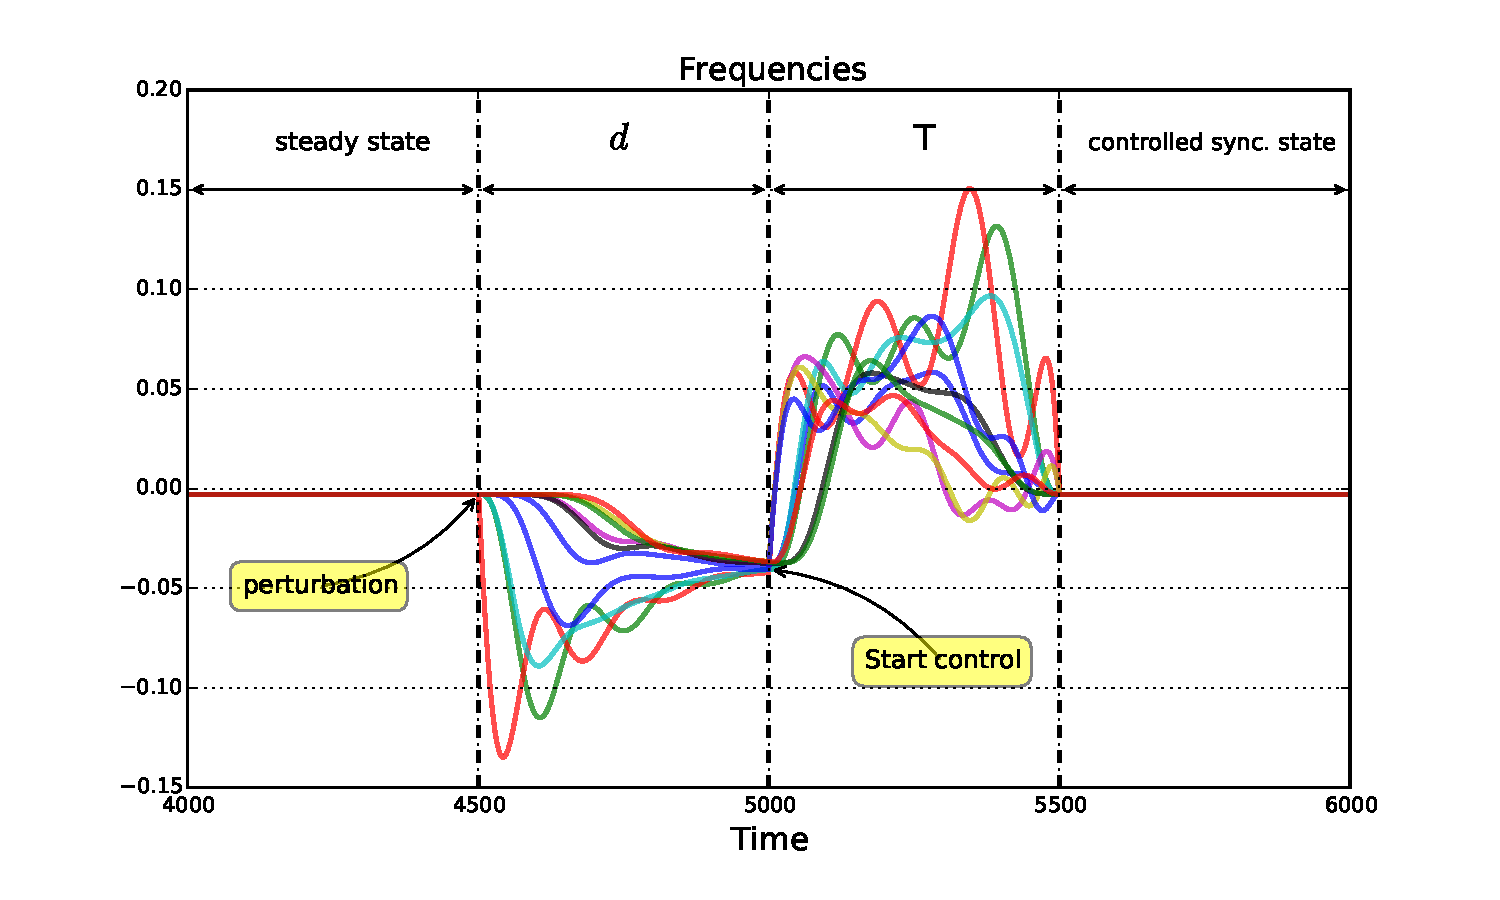
\includegraphics[scale=.38]{frequencies}
\caption{Time series of the N frequencies $\omega_i$ (phase angles are not shown for clarity). $d$ is the delay between the perturbation and the begining of the control phase that bring the system bak in the synchronized state in T time steps. Here, $d$ was chosen quite large for the clarity of the figure. Note that, if the perturbation is still active at this point, the system still needs control in order to stay synchronized (batteries should still compensate the power imbalance)}
\end{figure}

The purpose of selecting the drivers according to a Gramian related metric is to minimize, on average, the amount of control energy needed. In other words, if we select the drivers randomly, we expect to need, on average, more energy to control the system. In figure 2, we draw 200 example systems of 15 nodes with random topologies, power distributions, and line capacities. These systems are initially at equilibrium and are perturbed as explained previously. For each system we find the driver set S using algorithm (X) and we draw a random driver set $S'$ such that $S$ and $S'$ have the same size, and such that $S'$ also provide full control of the system. We then compute the control signals and the corresponding control energies $\mathcal{E}_S$ and $\mathcal{E}_{S'}$ for both $S$ and $S'$. Each system can therefore be represented as a point with coordinates $(|S|, \mathcal{E}_S)$. On figure 2, we plot the densities of these points for the random case (left pannel) and the optimized case (right pannel). Regions in dark red contains a lot of points while regions in dark blue have very few points. Figure 2 shows that most of the systems considered tend to be controlled by the drivers of algorithm X with less energy and/or drivers than for the random case.

\begin{figure}
\label{fig:densities}
\includegraphics[scale=.3]{rr}
\caption{test}
\end{figure}

We investigate next how the topology of the grid affects the size of the control set. We consider first the case of an erdos renyi topology with probability of connection p. We show on Figure 3 how the size of the driver set evolves with p for different Gramian based metrics and for two levels of constraints : 

\begin{itemize}
\item Level 1 : full control
\item Level 2 : full control + line capacities constraints + battery constraints (see algorithm X)
\end{itemize}

\begin{figure}
\label{fig:erdos_renyi}
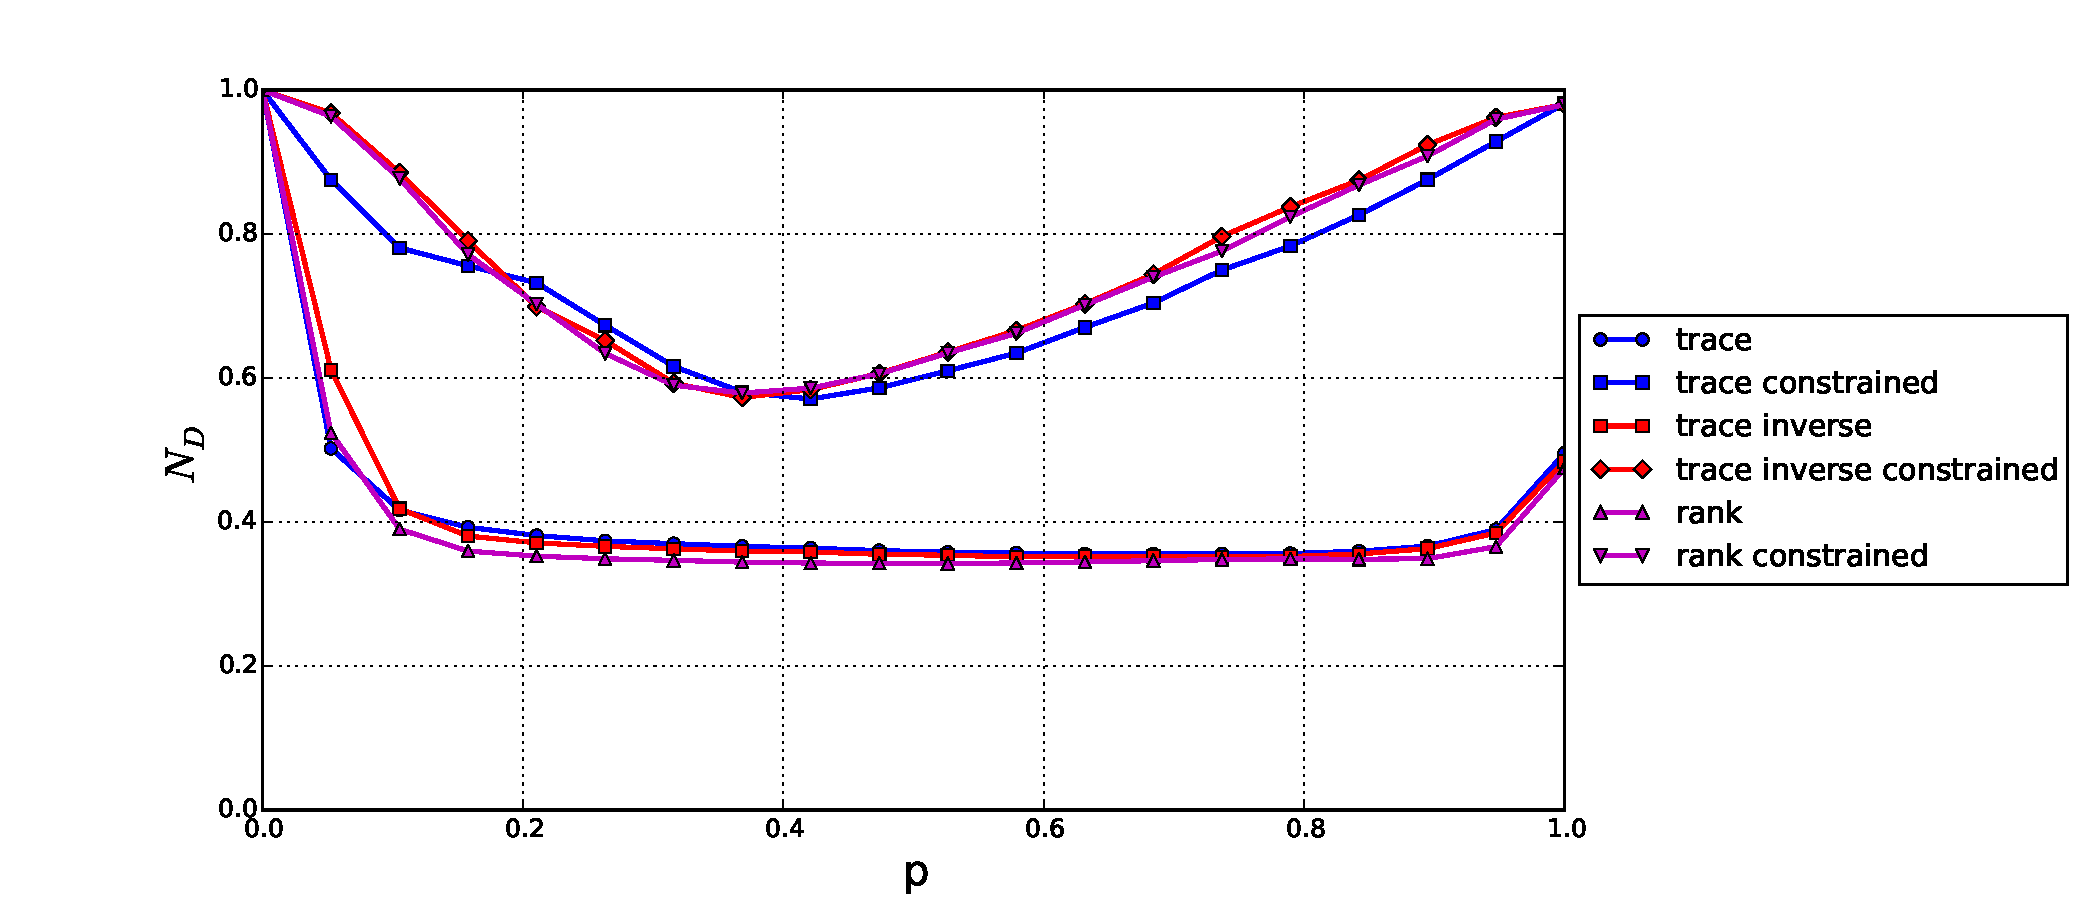
\includegraphics[scale=.3]{graphique_1}
\caption{ $ n_D $ against link probability p for erdos-renyi topologies ($ N=100 $). Curves are averaged over 100 realizations. The top three curves show the results for the three metrics taken into consideration when all constraints are considered (see Level 2 in the main text). The bottom three curves exhibit the results for the same metrics when only the full controllability constraint is considered (see Level 1 in the main text).}
\end{figure}


When p is close to zero, nodes tend to be very poorly connected such that we need to control almost all nodes in the grid. As p increases, the connectivity of the graph augments and the number of drivers decreases. At some point, the connectivity of the graph starts to harm its controllability, and more drivers are needed. This effect is in accordance with the litterature although it is less marked here because the topology has less influence in our model (recall that matrix A in the dynamics is not the adjacency matrix of the graph but a block matrix where one of the block is the Laplacian matrix of the graph). As expected, the driver sets for the level 2 of constraints are larger than for level 1 (for all metrics) because we impose far more constraints.



Because transmission power grids are spatially and politically constrained (each contry has its own transmission grid which is interconnected with neighboring grids at some specific locations), we study the control in clustered graphs. More precisely, we use a block model $(N, N_{clusters}, p_{in}, p_{out} ) $ to generate random topologies where $ N $ is the number of nodes, $N_{clusters} $ is the number of clusters, $p_{in} $ is the probability that two nodes within the same cluster are linked, and $ p_{out} $ is the probability that two nodes in two distinct clusters are connected.

\begin{figure}
\label{fig:block_model_1}
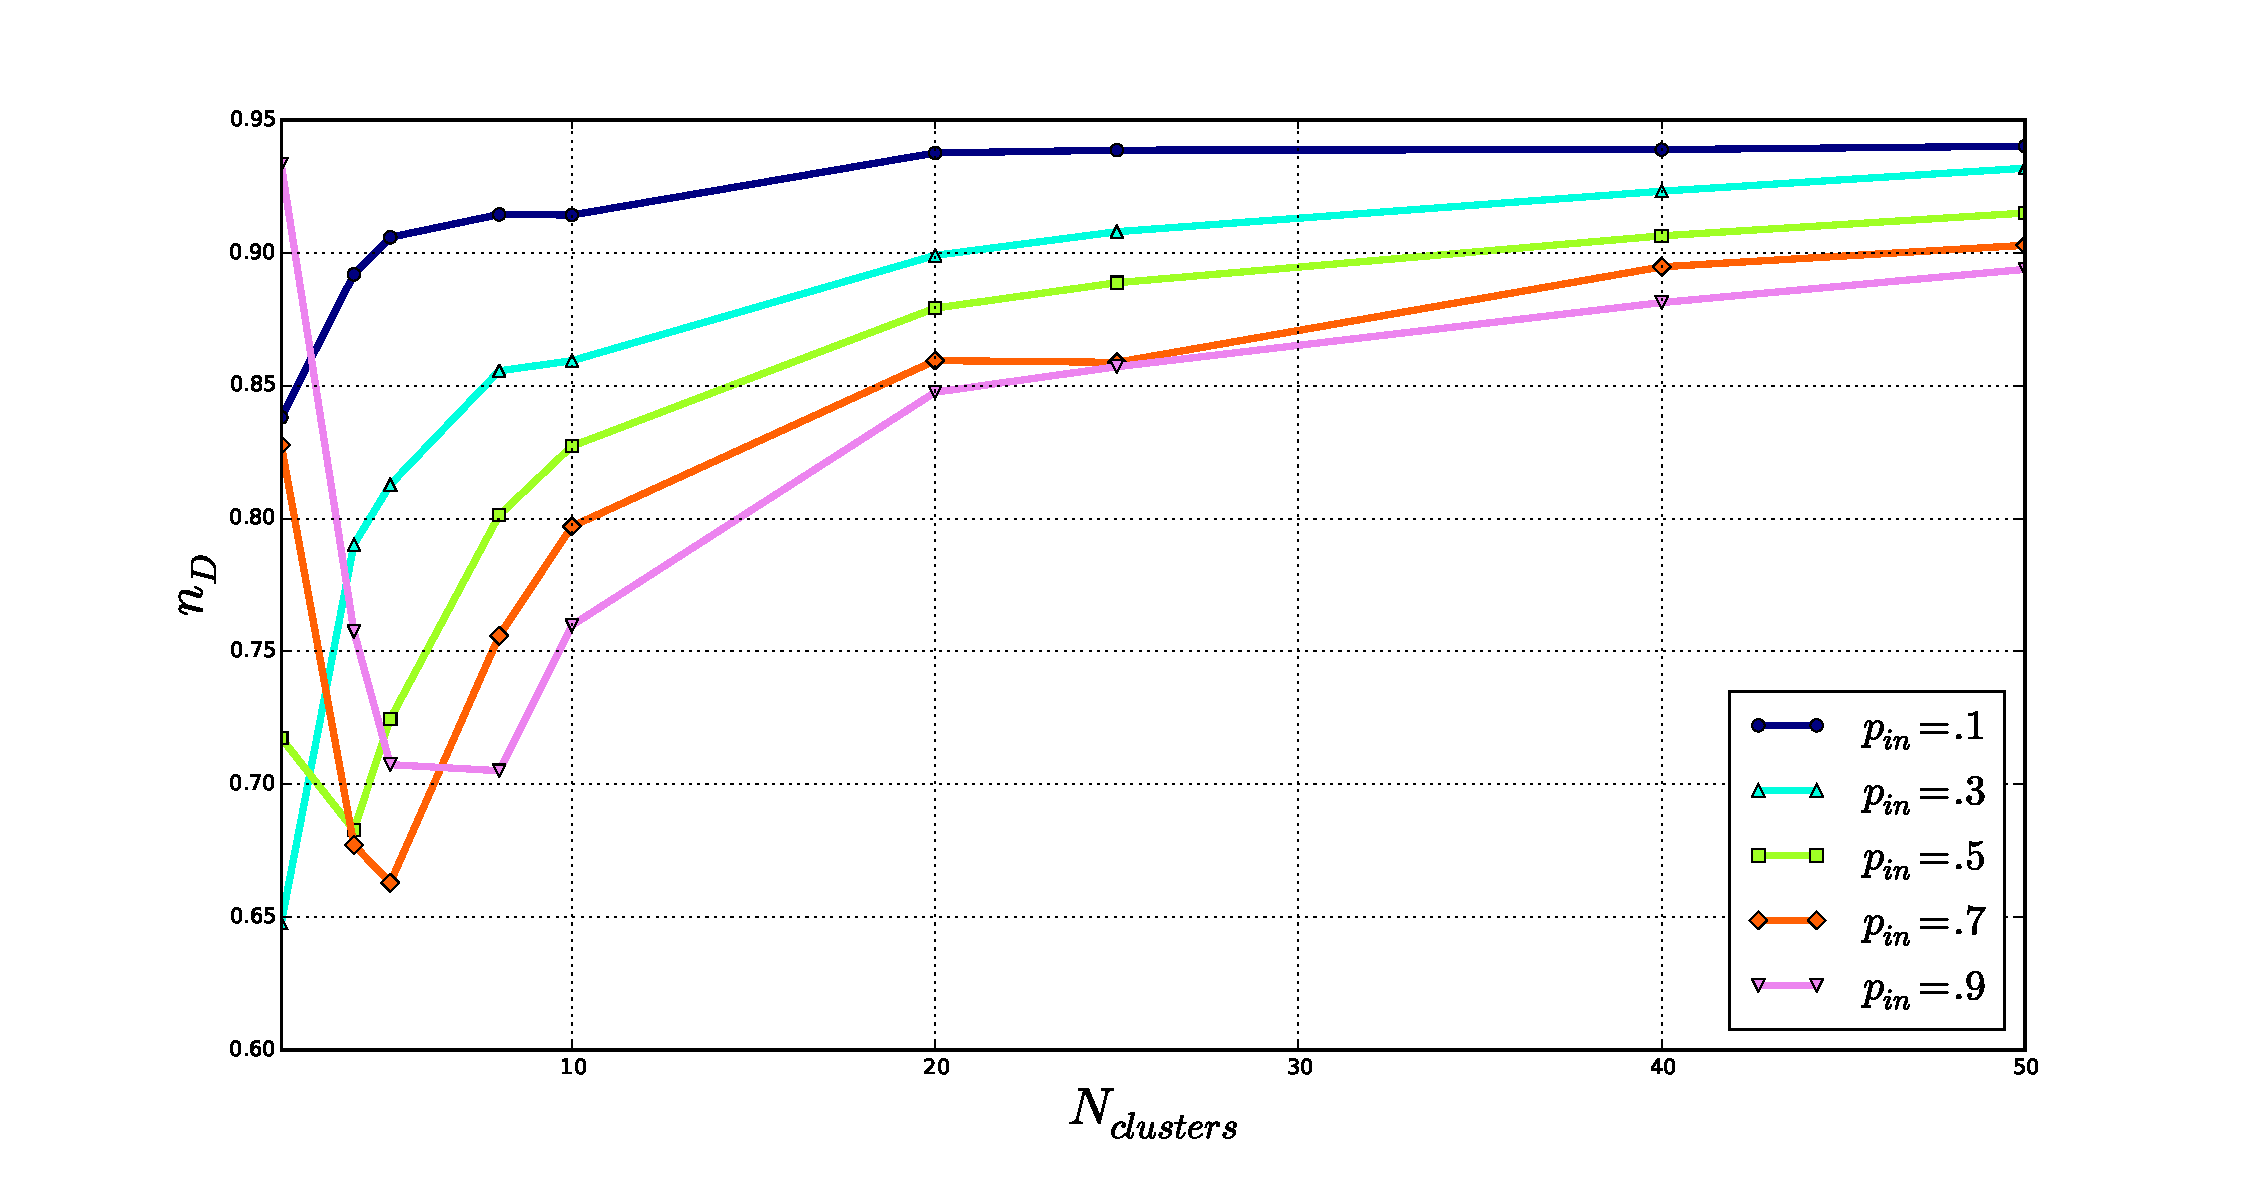
\includegraphics[scale=.25]{block_model_3}
\caption{$n_D$ against $N_{clusters} $ for different values of $ p_{in} $ and $ p_{out} = 0.1 $. $ N=200 $ and curves are averaged over 100 realizations.}
\end{figure}

Figure 4 shows how the number of drivers evolves with the number of clusters for different values of $ p_{in} $ when $ p_{out} $ is fixed ($p_{out} =0.1$). For small values of $ p_{in} \sim p_{out} $ clusters are poorly marked, and the connectivity is low. The number of drivers in these conditions is large and increases slowly when the number of clusters augments. As $ p_{in} $ increases, the clusters becomes more densily connected such that within a cluster less drivers are required in order to control it. As the number of clusters grows, more drivers are required. For large values of $p_{in} $, the behavious is more complex. We see indeed that for $p_{in} = 0.9 $ and $N_{clusters} = 2$, almost $ 94\% $ of the nodes are needed for control, but this quantity first decreases with the addition of a few more clusters ($ 71\% $ for $ N_{clusters}=5 $), before increasing. This behavior can be explained by the fact that controlling a very dense network requires, in our settings, a very large portion of nodes to be drivers. Controlling one cluster alone thus requires to control almost all nodes within this cluster. Nevertheless, when a relatively small (compared to the number of nodes in the graph) number of clusters are interconnected with a few links, nodes in one cluster are able to control nodes in other clusters to which they are connected. As the number of clusters grows, the global connectivity increases rapidely, such that the number of drivers also rises. We show this behavior in more details in figure 5, where the number of drivers is plotted against $ p_{in} $ for $N=200$ and $N_{clusters} \in \{2,4,5\} $. For $N_{clusters} = 2 $ and $ p_{in} = 0.1 $ the number of drivers is large since the graph is poorly connected. When $p_{in} $ increases, $n_D$ decreases until a minimum value $n_D \sim 0.64 $ at $ p_{in} \sim 0.6 $. After this point, $n_D$ augments with $p_{in}$. For $N_{clusters} = 5 $, we do not see this behavior : $ n_D $ decreases continuously as $p_{in} $ increases as expected from the curves of figure 4.


\begin{figure}
\label{fig:block_model_2}
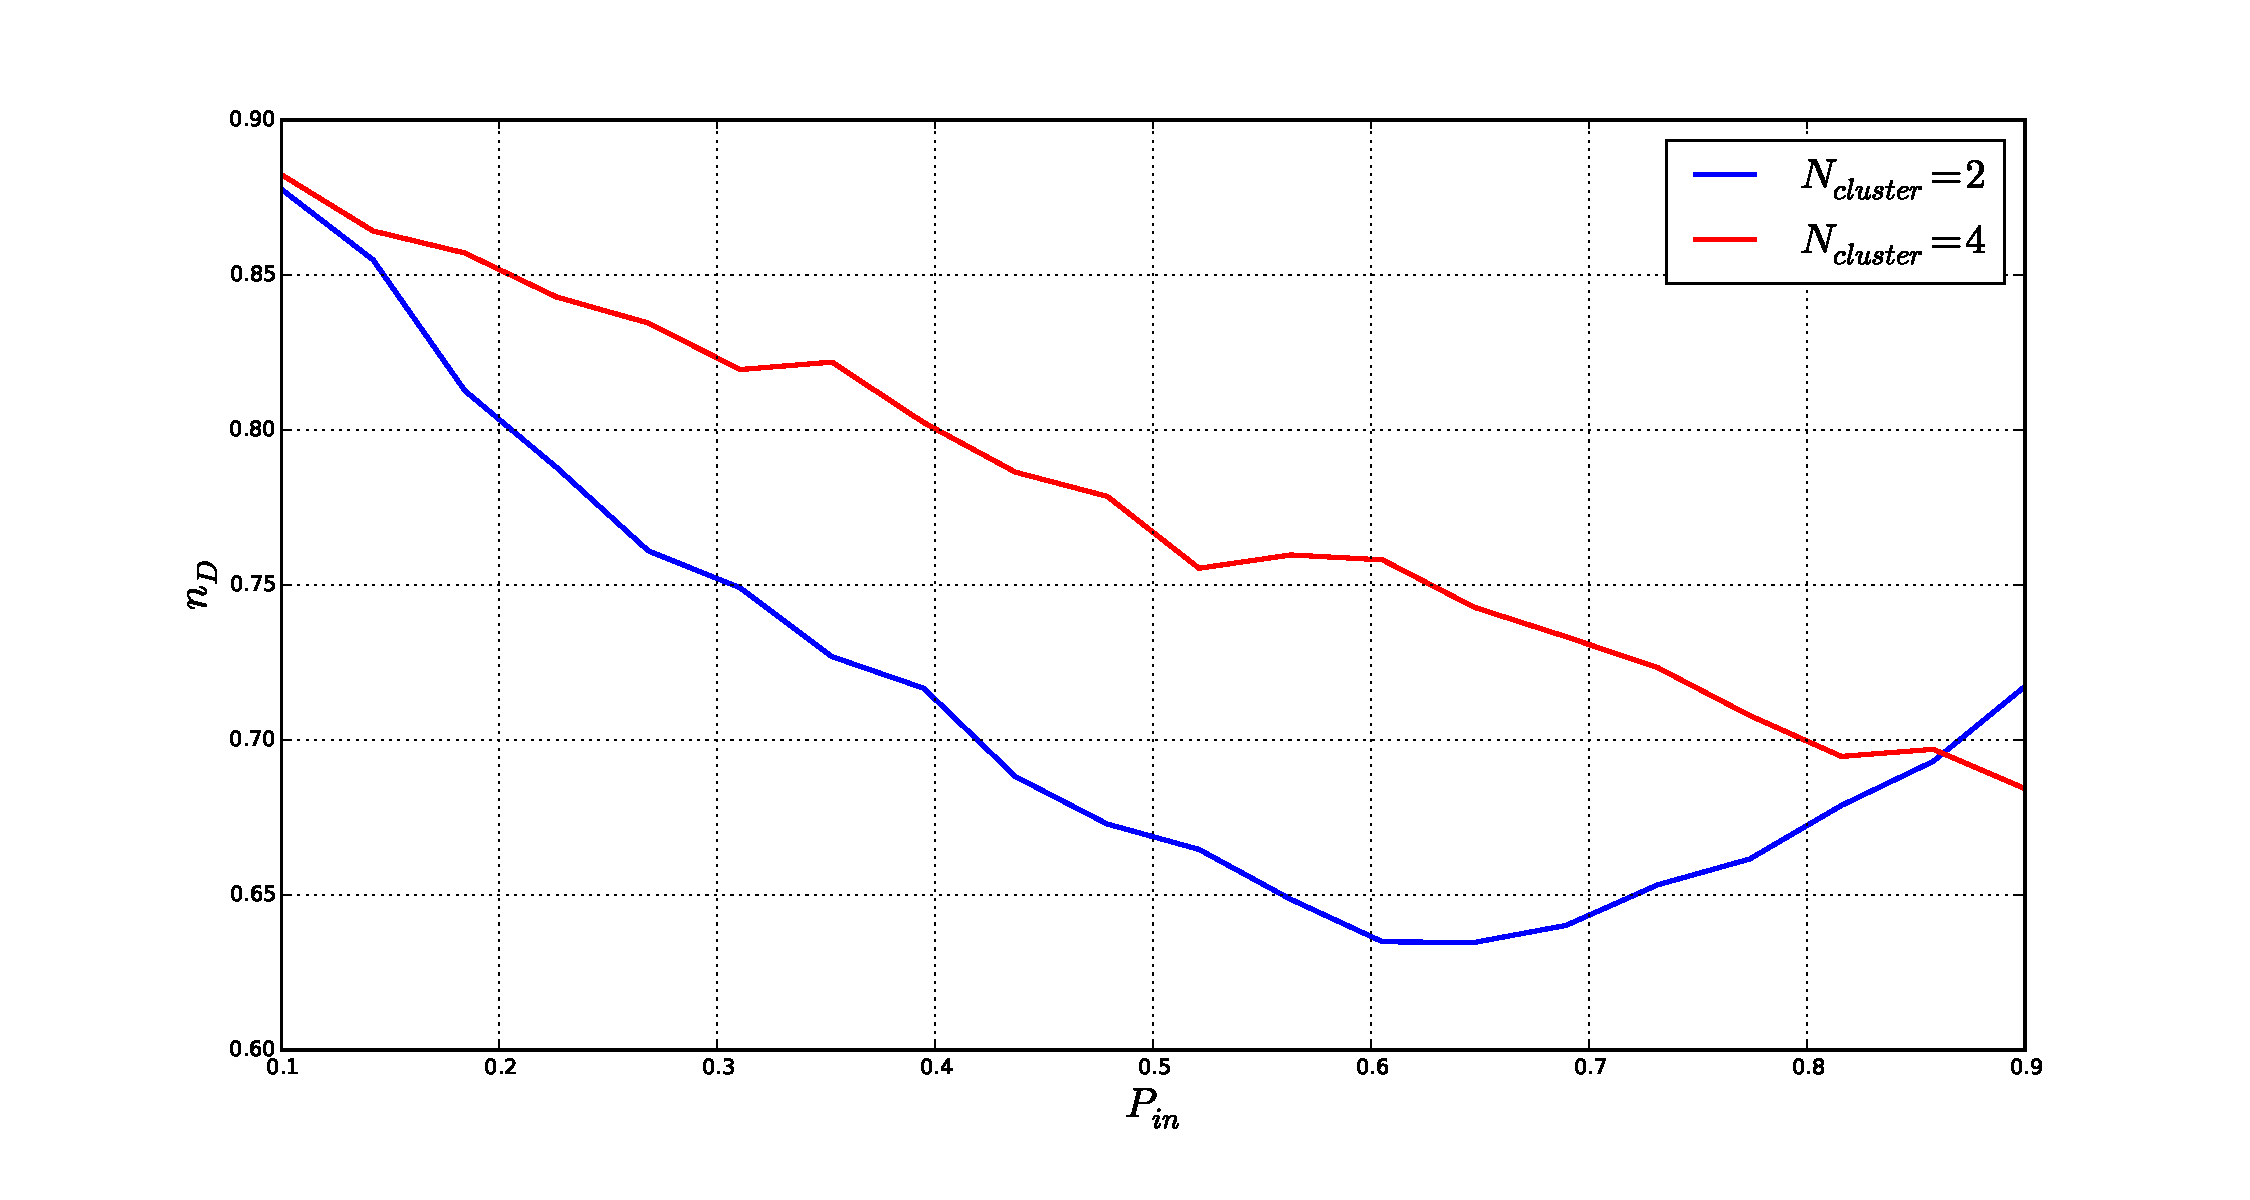
\includegraphics[scale=.25]{block_model_4}
\caption{$n_D$ against $ p_{in} $ for systems of $N=200 $, $p_{out} = 0.1 $, and for different values of $N_{clusters} $. The curves are averaged over 100 realizations.}
\end{figure}


Until now, we have considered all batteries to be equal, i.e they have the same capacity and charge/discharge rate. Although simple, this assumption might not be verified in practice where different types of batteries exist. Making a cost-oriented study where the location os various types of batteries is studied such that the tradeoff between costs and reliability is out of the scope of this paper. Nevertheless, we studied how the number of drivers behaves when the batteries have different capcities. More precisely, we draw the capacities of the batteries from a normal distribution $ \mathcal{N}( \mu_{\lambda}, \sigma_{\lambda} ) $ and keep a simple erdos-renyi topology for the power grid. Note that each node is assigned a capacity regardless of its caracteristics (degree, betweeness, and so on...). In figure 6, we plot $n_D$ as a function of the relative standard deviation of the battery capacity distribution $ \sigma_{\lambda} / \mu_{\lambda} $. We see that $n_D$ increases with the variance of the capacity distribution for all three gramian based metrics considered. Moreover, this rise is abrupt since $n_D$ goes from $ 60 \%$ for $\frac{\sigma_{\lambda}}{\mu_{\lambda}} \sim 0.15 $ to $100 \% $ for $\frac{\sigma_{\lambda}}{\mu_{\lambda}} \sim 0.27 $. 

\begin{figure}
\label{fig:batteries_variance}
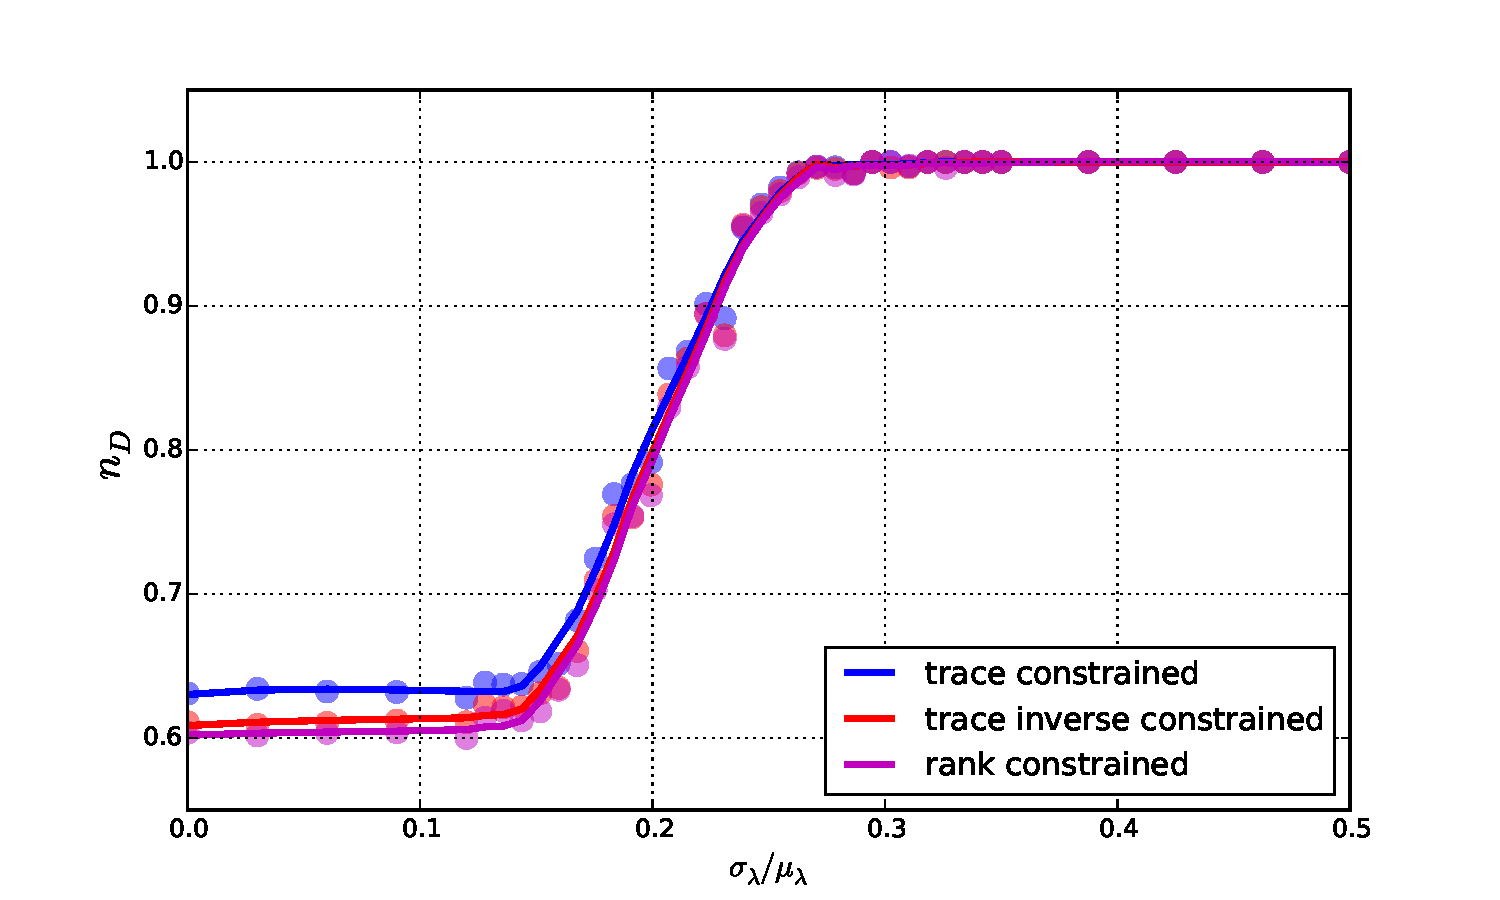
\includegraphics[scale=.37]{batteries_variance}
\caption{$n_D$ against the relative standard deviation of the capacity distribution of the batteries $ \frac{ \sigma_{ \lambda } }{ \mu_{ \lambda} } $. The dots are averages over 100 realizations and the curves are obtained using a Savitzky-Golay filter, each color shows the results for a given metric. The graphs are erdos-renyi with $N=100$ and $p=0.3$, and $\mu_{\lambda} = 100 $ units. }
\end{figure} 

Real power grids topologies are known to be far from random such that using the erdos-renyi model probably do not give a realistic insight into the control of these systems. Depending on the voltage level 

In this section, we provide some results in order to illustrate the work described above. We use a small 10 prosumers example, connected with a random topology. The line maximum capacities are selected  according to a normal distribution $\mathcal{N}(\mu_l,\sigma_l)$.  The power distribution is chosen as a zero mean normal distribution $ \mathcal{N}(0,\sigma_p) $, and the samples should satisfy the constraints \ref{synchro_constraint} and \ref{zero_sum_constraint}. Obviously, $\mu_l$, $\sigma_l$, and $\sigma_p$ should be chosen such that, without any perturbation, the lines are not already overloaded.



Once the synchronized state is reached, we apply a perturbation to the power distribution such that there is a mismatch between production and demand (constraint \ref{zero_sum_constraint} is not satisfied). We denote by $d$ the delay between the perturbation and the start of the control phase (see figure \ref{fig:frequecies}). $d$ depends on how fast the perturbation can be identified and located, the control inputs calculated and communicated without error through the communication network.


 If the driver set is fixed, we expect that the higher $ d$, the higher the control energy required to drive the system back to the synchronized state. Eventually, if $d$ is too large, the minimum energy control inputs will result in some constraints being broken (battery levels, line flows, and so on...).

\begin{figure}
\label{fig:energy_vs_delay}
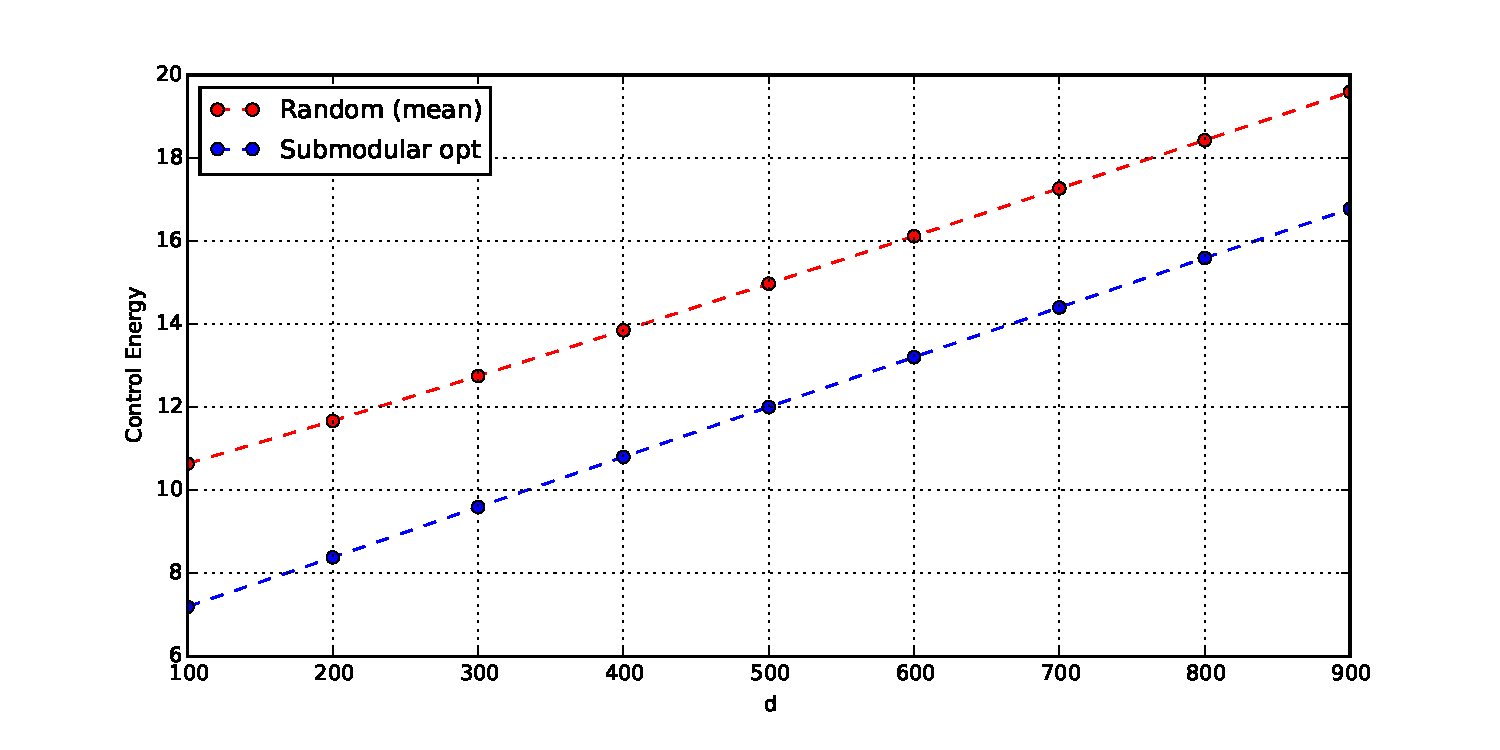
\includegraphics[scale=.38]{energy_vs_delay2}
\caption{ Control energy used in order to bring the system back to the synchronized state when the delay between perturbation and control increases, while the driver node set is fixed. The blue dotted curve shows the results for $ S_k^{\star} $ our algorithm \ref{algo_1}. The red line shows (average and standard deviation) the results when the driver set is sampled uniformly from all possible sets of the size $ k $.}
\end{figure}

As visible on figure \ref{fig:energy_vs_delay}, when d increases, the system deviates more from the equilibrium and this results in more energy being used to steer it back to synchrony. We also investigate here how the driver node set selected with algorithm \ref{algo_1} performs against other driver sets of the same size. we use a Monte-Carlo sampling of the drivers sets of the same size as our solution, and filter out the ones that do not meet all the constraints. Figure \ref{fig:energy_vs_delay} shows that our solution (blue dotted curve) uses less energy than other driver sets of the same size (red curve).


\section{Conclusion}
\label{sec:Conclusion}
C'est fini !



\bibliographystyle{IEEEtran}  
\bibliography{Article}

\end{document}

